As was already noted in the previous chapter, \ac {NN} can be both acyclic and cyclic graphs. The
\emph{vanilla} \ac {NN} is usually considered to be a acyclic feed-forward network, as it has no internal state and is
therefore more suited to describe the concepts of how the networks operate. Especially in translation and text to speech
applications though, \ac {RNN} are very popular as they are able to act on previously seen information in a sequence of
data. Generally they are suitable for many applications where the data has some kind of time-dependent embedding
\cite[p.373]{Goodfellow-et-al-2016}.

A \ac {RNN}, therefore computes its output based on the weights $w_i$, commonly noted as $\theta$, it's current input
$x^t$ and it's previous hidden units internal states $h^(t-1)$.

\[
    h^t = f(h^(t-1), x^t, \theta)
\]

The network generally learns to use $h^t$ to encode previously seen aspects relevant to the current task, although this
is inherently lossy as the previous number of inputs (i.e. $\mid t-1\mid$) is arbitrary. Figure~\ref{fig:rnn_concept}
shows this concept.

\begin{figure}[]
    \centering
    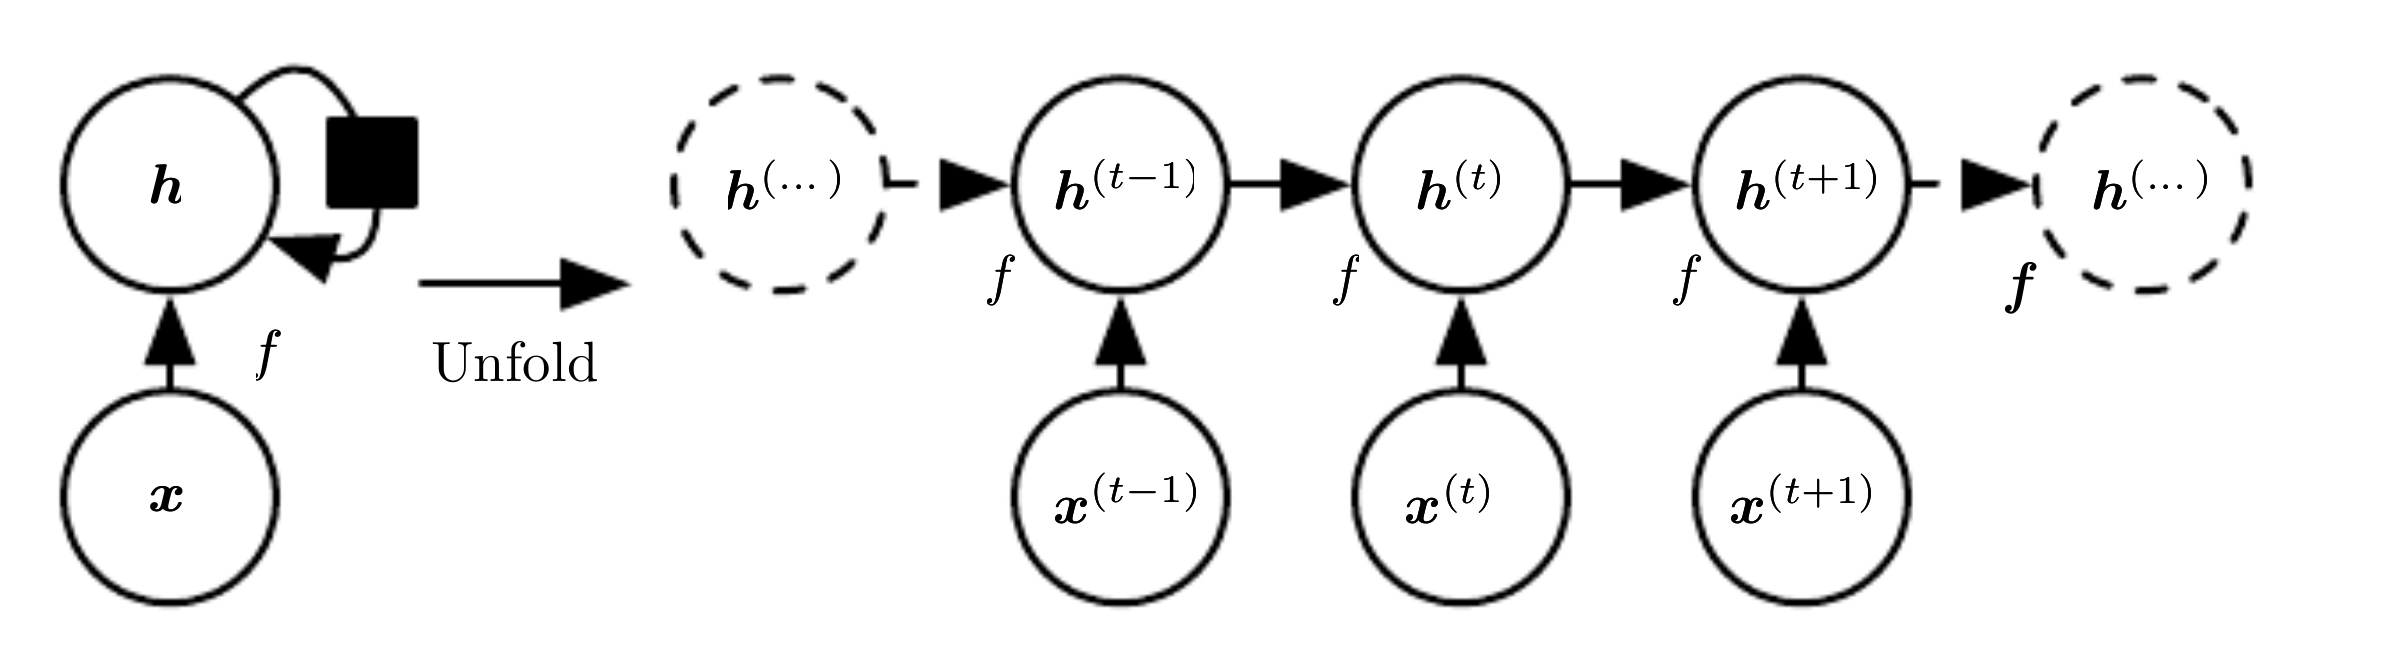
\includegraphics[width=0.8\linewidth]{img/rnn_concept.png}
    \caption{A recurrent neural network conceptualized. \emph{Left}: Circuit diagram where the black square represents a
    1 time-step delay. \emph{Right:} The same network unfolded where each node represents a particular time instance.
    Taken from \citet{Goodfellow-et-al-2016}.}
    \label{fig:rnn_concept}
\end{figure}

The network structure has two benefits: Firstly, it allows for arbitrary sequence length, as the network size is
dependent on the time-step specific input and not on the number of previous timesteps. Secondly, the same network with
the same weights (or in mathematical terms the same transition function $f$) can be used during each time-step. This
means: When a \ac {RNN} is fed a sequence of data, the weights will stay the same throughout the sequence. They can be
updated after the entire sequence has been processed. 
